\subsection{Command Class Implementation} 
 
Z-Wave device functions are controlled by command classes. A command class can be have one or  multiple commands
allowing the use of a certain function of the device. Command classes are organized by functions, e.g. the command class "Switch Binary" allows to switch 
a binary switch. Hence the number of supported command classes defines the functionality and the value of 
a device.

Z-Wave defines quite a few command classes but a lot of them are not implemented in any device. Hence, Z-Way will not implement them 
either. Command Classes consist of two types of commands:
\begin{itemize}
\item commands for users, most of them are either "GET" commands asking for a value or status from a remote device, or they are "SET" commands setting
 a certain value and therefore causing a certain action.
\item commands for configuration
 \end{itemize}

The commands for configuration are used by Z-way to build the data model used and to manage the device itself but they are not made public for users. 
The command classes available for users are listed in chapter \ref {ccs}.

Commands to Z-Wave devices take time to be executed. In case the device is awake (mains powered or FLIRS) the delay may be well below one second but for 
battery powered  devices the controller has to wait for the next scheduled wakeup in order to send the command. 

In case the command is calling a value update from e.g. a sensor the successful execution of the command only means that the request was accepted by the
wireless device. In order to really update a value the device itself needs to send a wireless command back to the controller that needs to be accepted by the 
controller.    

Each data element that is available in a remote wireless device (e.g. a switch) is also stored in  Z-Way. First of all there is the assumption that the data value of the remote device
and the corresponding data value in Z-Way are identical.

 Most commands of command classes are eighter a "GET" asking for an update of an value or they are a "SET" - setting a new value. Setting a new 
 value may also cause an action on the remote side. As an example switching a binary switch means in Z-Wave command classes changing the switching  
 state value wirelessly.

Z-Way will never "just" update the local corresponding value of the real remote value but always ask the remote device after a successful "SET"  command for 
an update of the remote value using a "GET" command.  This means that the local  - displayable - value of a certain remote device will only update after some delay.

The process can be examined using the "Device Control" dialog in the demo user interface.

 
\subsubsection{Switch Overview}



\begin{figure} 
\begin{center}
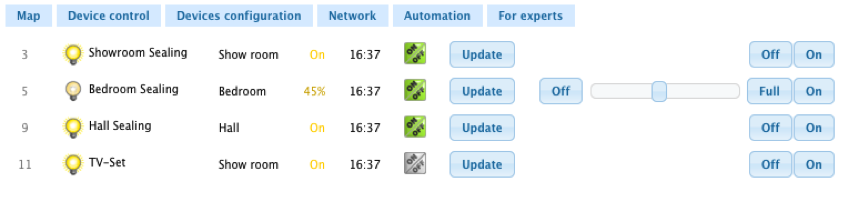
\includegraphics[scale=0.8]{pics/switches.png}
\caption{Demo UI Dialog for Switches}
\label{c3:demosen} 
\end{center}
 \end{figure}
This page gives a table style overview of all actuators of the Z-Wave network. Actuators are devices with some kind of switching function such as 

\begin{itemize}
\item Digital (on/off) switches, 
\item Light Dimmer, 
\item Motor Controls for Venetian blinds, window bind,
\item Motor Control to open/close doors and windows.
\end{itemize}

Beside the name of the device, the location and the type of device the actual status and the timestamp of this status are shown.

Of course it is possible to switch the devices and to update the status of the device.

A little icon indicates how the device will react to a “switch all devices” command  (will switch, will 
not switch, will react to off command only or to on command only).

The commands to control the different actors apply the  command classes "Switch Multilevel" and "Switch 
Binary". Please refer to Chapter \ref{ccs} for details how to use these command classes.


\subsubsection{Sensor Overview}


\begin{figure} 
\begin{center}
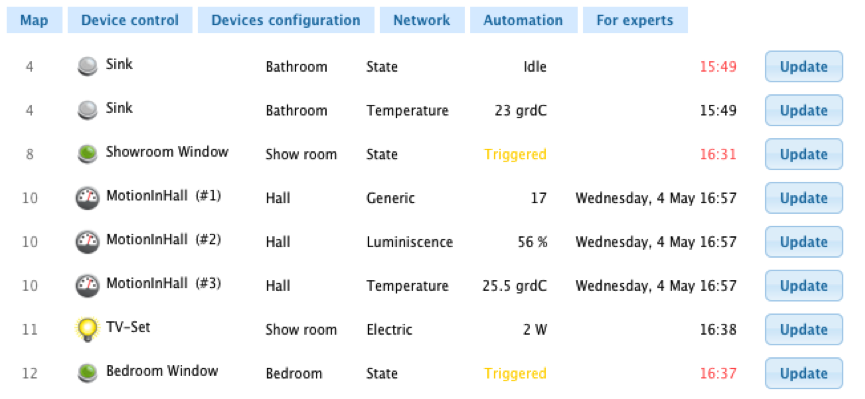
\includegraphics[scale=0.5]{pics/sensors.png}
\caption{Demo UI Dialog for Sensors}
\label{c3:demosensor} 
\end{center}
 \end{figure}

 This page gives a table style overview of all sensors of the Z-Wave network.  
Sensors are devices able to report measured values. Sensors can report binary or analog values.  Beside the name of the device, the location and the type of sensor the actual sensor value and the timestamp of this value are shown. It is possible to ask for an update of the sensor value.

 
 
The update command of the sensor interface and  the values shown are using the command classes "Sensor Multilevel" and "SensorBinary". Please refer to Chapter \ref{ccs} for details how to use these command classes.
 
\subsubsection{Meter Overview}

This page gives a table style overview of all meters of the Z-Wave network.  
Meters are devices able to report accumulated values.  Beside the name of the device, the location and the type of meter the actual meter value and the timestamp of this value are shown. It is possible to ask for an update of the meter value.
 
The update command of the meter interface and the values shown are using the command class "Meter". Please refer to Chapter \ref{ccs} for details how to use the meter command class.

\subsubsection{Thermostat Overview}

This page gives a table style overview of all thermostats of the Z-Wave network.  
Depending on the thermostat capabilities reported, the dialog will allow to change the thermostat mode and/or change the setpoint temperature 
for the thermostat mode selected.
 
Please refer to Chapter \ref{ccs} for details how to use the thermostat setpoint and thermostat mode command classes.

\subsubsection{Door Lock Overview}

This page gives a table style overview of all door locks of the Z-Wave network.  
Depending on the door lock reported, the dialog will allow to open/close the door
and differentiate on door handles.
 
Please refer to Chapter \ref{ccs} for details how to use the door lock, user code
and door lock logging command classes.


 
 
\subsubsection{Device Configuration} 
 
Beside the command class to directly control devices and update device values there are more 
commands that are used to built the data model of the device and to get configuration values. 

The device also allow certain configurations itself. The demo UI shows the use of these command classes in the Tab "Device Configuration". The device configuration fulfills three basic tasks:

\begin{itemize}
\item The interview process after inclusion of the device
\item The configuration of the device according to user requirements and needs.
\item Setting Cause/effect relationships. This means that certain devices can directly control other devices.

\end{itemize}


\subsubsection{Interview Process}
After the inclusion of a new device Z-Way will interview this very device. The interview is a series of commands Z-Way is sending 
to the device in order to learn the capabilities and functions of this device.


Depending on the capabilities announced in the Node Information Frame that was received during the inclusion, Z-Way will ask further 
questions to get more detailed information. The interview process may take some seconds since more questions may be required to ask depending in certain answers given.
Since all functions of a device are grouped in so called Command Classes each command class announced in the Node Information frame will typically cause its part of the interview.
The interview will be executed in three different steps:

\begin{enumerate}
\item In case there is a Version Command Class ask for the Version of the device and the versions of all Command Classes announced in the Node Information frame. Otherwise Version 1 is assumed.
\item In case there is a Multi Channel Command class announced, ask for the number of the capabilities of the different channels and repeat Step 3 for each channel.
\item Ask for all capabilities of all command classes.
\item Do some auto configurations if needed.
\end{enumerate}

The „Device Status“ tab will indicate if the interview was successfully completed.  The blue information icon shows if the interview was not complete. Clicking on this icon opens a dialog with all command classes and the status of their respective interviews.  
A complete interview is important in order to have access to all functions of the device included. Incomplete interviews may also be a reason for malfunctions of the network.
There are several reasons why an interview may not be completed.
\begin{enumerate}
\item A battery-operated device may be gone into sleep mode too early. In this case it is possible to wake up the device manually to complete the interview. Sometimes manual wakeup is needed several times.
\item The device does not fully comply with the Z-Wave protocol. This is particularly possible for devices that were brought to market before 2008. 
The current more sophisticated certification process makes sure that devices are 100\% compatible to the Z-Wave product when they hit the market. 
Please check online ressources on wikis and forums for further details and possible ways to fix these kinds of problems.
\item The device does not have a reliable communication route to the controller. Interview communication typically use longer packets than normal polling communication. This makes the interview communication more vulnerable against weak and instable communication links. Its possible that the controller is able to include a device and even receive confirmation of a polling request but still not being able to complete the interview. However this is a rare case.
\item The device may be simply broken.

\end{enumerate}

Most of the command exchange during interview is using commands dedicated for the interview process. They are not exposed on the API.

\subsubsection{Device Configuration} 


Each Z-Wave device is designed to work out of the box after inclusion without further configuration. 
However, it may be suitable and in certain contexts even required to do a device specific configurations.

The device configuration page allows to further configure the device and to access certain additional 
information about the device. The tab is grouped into several sections. The sections can be toggled 
from invisible to visible and back by clicking on the headlines:
\begin{itemize}
\item Select Z-Wave Device Description Record
\item Device Description
\item Configurations
\item Actions with configurations
\item Advanced Actions
\end{itemize}

\paragraph{Select Z-Wave Device Description Record}

After a successful inclusion Z-Way will interview the device to gather further information.  

Certain information such as names of association groups, the brand name of the device and the parameters of further configuration values can not be detected during interview. 
Z-Way uses a device database with product description files to obtain this information. In order to identify the right device description record, certain parameters of the interview are used. 
If these parameters match exactly one device description record, this very record is loaded and its content is shown on the device configuration page automatically.

If the information from the device is sufficient to select one specific record from the database this section of the tab is hidden. 
If it is not possible to identify the correct device description record the user can manually choose the correct record. It is also possible to manually 
change the selection of the device description by unhiding this section and clicking on the “Select Device Description Record” button.

\paragraph{Device Description}

The upper part of the dialog shows some descriptive values of the device.  The Z-Wave device type is the only value generated solely from the interview data. All other data are taken from the device description record.
\begin{itemize}
\item Zone: ... the zone/room the device is assigned to. Will be manually defined in Zone-tab.
\item Brand: … the product code or brand name of the device. This will be taken from the device description record.
\item Device Type: ... the type of Z-Wave device as reported by the device during inclusion.
\item Description: … a verbal description of the function. This will be taken from the device description record.
\item Interview Stage: …shows the progress of the interview process. This information is generated by Z-Way.
\item Inclusion Note: … how to (re-) include the device. This will be taken from the device description record.
\item Wakeup Note: … this will be taken from the device description record.
\item Documents: … If the device description record offers links to manuals or other online documents there are shown here. This will be taken from the device description record.
\item Device State:  Status of the device plus number of packets queued for this device
 \end{itemize}

\begin{figure} 
\begin{center}
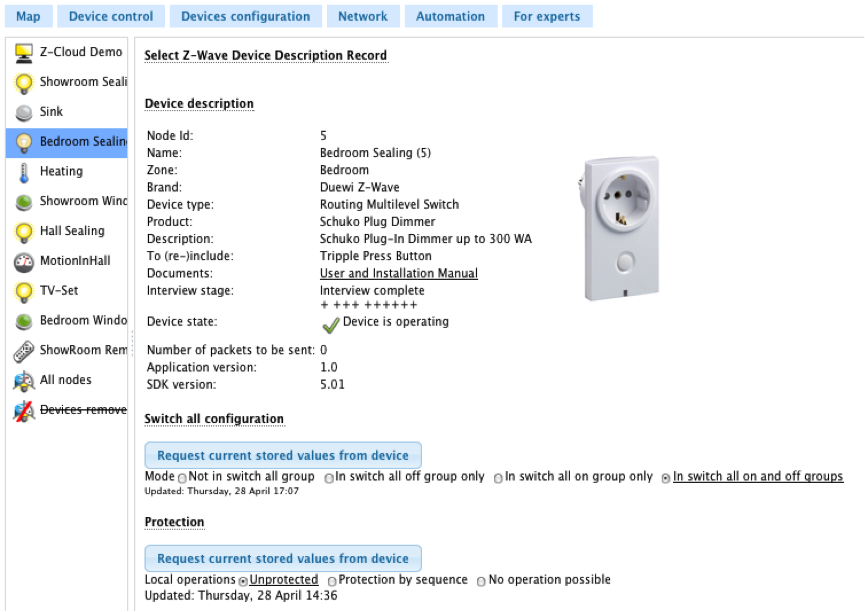
\includegraphics[scale=0.7]{pics/dconfig.png}
\caption{Demo UI Dialog for Sensors}
\label{c1:demosensors} 
\end{center}
 \end{figure}


There are a couple of reasons why no device description record was found:
\begin{enumerate}
\item There is no record for the device available. Since there are always new devices on the market Z-Way needs to catch up and update its device database. If your device is not found, updating to the most recent version of Z-Way may help.
\item The interview was not finished to the point where enough parameters were detected to identify the correct device description record. You may manually choose the correct device description record using the button “Select Device Description Record”. A dialog box will be opened for manual selection of the product (if available). The manual selection of a device description record is only needed if no record was found on default.  
\item The interview of the device was completed but the device does not offer enough information to identify the correct device. You may manually choose the correct device description record using the button “Select Device Description Record”. A dialog box will be opened for manual selection of the product (if available). The manual selection of a device description record is only needed if no record was found on default.
\item There is more than one device description record matching the information gathered during interview.  This is particularly possible if a vendor sells devices with different firmware and functions without properly updating the firmware version information. You may manually choose the correct device description record using the button “Select Device Description Record”. A dialog box will be opened for manual selection of the product (if available). The manual selection of a device description record is only needed if no record was found on default.
\end{enumerate}

\paragraph{Device Configuration}

This section will, if device description record is loaded,  show device specific configuration values including their possible parameters and a short description of the configuration value. You may change these values according to your needs.

\paragraph{Actions with configurations}

The most important action in regard to the configuration is to apply the configuration to the device. This is only done when the button “Apply configuration for this device” is hit. This button is therefore even shown, when the rest of the tab part is hidden.
\begin{itemize}
\item Mains Powered Devices: The settings will become effective immediately after hitting the button.
\item Battery Powered Devices: The settings will become effective after the next wakeup of the device, as shown in the Device Status tab.
\item Battery Powered Controllers (remote controls or wall controllers): The settings will only become effective if the devices are woken up manually. Refer to the controller manual for more information on how to wake up the device. Appendix B may also give further advice.
\end{itemize}

If there are many similar devices in a network, it is desirable to just apply one working configuration to all these devices. This can be done using the function 'Copy from other Device'.

The set of defined configuration values is stored for every device. Therefore its possible to pick a different device and reuse its configuration values for the device to be configured.  
The „Save“ function of the bottom context menu allows saving the configuration for further use and reuse.

\paragraph{Actions with configurations} 

This function requests the selected device to send its Node Information frame (NIF) to the controller. It can be used instead of triple pressing a button on the device itself that would also instruct the device 
to send it NIF. The NIF is needed to know device capabilities.

\paragraph{Delete Configuration of this device – in section “Actions with configuration”}

This function deletes the stored configuration for this device. This function is for debugging purposes only.

\paragraph{Force Interview – in section “Advanced”}

This functions forces to redo the whole interview. All previous interview data will be deleted. This function is for debugging purposes only.

\paragraph{Show Interview Results – in section “Advanced”}

This function shows the result of the interview. This function is for debugging purposes only. For information about reasons for incomplete interview please refer to the manual section “Device Status”.

The bottom context menu function  „Reset Configuration“ deletes all configurations stored in Z-Way, but does not affect devices!



The configuration dialog documents the use of the command classes "Association", "Protection", "Configuration" and "Switch All".
  
\subsubsection{Associations}


If there was no previous device of the same type installed, the interface will show the values as read from the device. If there was already a device of the same kind installed, there may exist a stored default configuration for this particular device. Then the setup in the device may differ from the default configuration stored in Z-Way.
\begin{itemize}
\item Gray Icon: This Node ID is stored in the device but its not stored in the default configuration of the Z-Way. You can double click this device to store this setting in the Z-Way default configuration of this device type.
\item Red Icon: This Node ID is stored locally but not in the association group of the device yet. Apply the settings to transmit the setting into the device.  In case of a battery operated device you need to wakeup the device in order to store the configuration.
\item Black Icon: This Node ID is stored both in the device and in the local configuration of Z-Way.
\end{itemize}
Hint: The auto configuration function of Z-Way will place the node ID of the Z-Way controller in all association 
groups if possible. This allows the activation of scenes from these devices. 

All management of Associations is handled by the command class "Association", In case the target device is a multi 
channel device the command class "Multi Channel Association" is used. Please refer to capter \ref{ccs} for details how to use these command classes.




